\documentclass[12pt, a4paper]{article}
\usepackage{enumitem}
\usepackage{float}
\usepackage[left=2cm, right=2cm, top=2cm, bottom=2cm]{geometry}
\usepackage{graphicx}
\usepackage[colorlinks, urlcolor=blue]{hyperref}
\usepackage{xeCJK}

\renewcommand\arraystretch{1.1}
\setCJKmainfont[AutoFakeBold=1.5]{新細明體}

\title{
  \vspace{-1cm}
  Network Administration/System Administration\\
  (NTU CSIE, Spring 2024)\\
  Homework \#6 - OPNSense
}
\author{\Large B12902110 呂承諺}

\begin{document}
  \maketitle
  \section*{Short Answers}
  \begin{enumerate}
    \item ``Block" drops traffic silently, while ``Reject" notifies the client with a
    TCP RST packet or a UDP ICMP UNREACHABLE packet. ``Block" is more suitable on WAN
    interfaces, so that to external attackers it appears as if there is nothing. ``Reject"
    is more suitable on LAN interfaces, so that clients don't have to wait for timeouts.

    \textbf{References}
    \begin{itemize}
      \item \href{https://docs.opnsense.org/manual/firewall.html}{Rules — OPNsense  documentation}
      \item \href{https://en.wikipedia.org/wiki/Transmission_Control_Protocol}{Transmission Control Protocol - Wikipedia}
      \item \href{https://forum.netgate.com/topic/56854/reject-block-what-s-the-difference}{Reject | block What's the difference ? | Netgate Forum}
    \end{itemize}

    \item The ``interface net" refers to the entire subnet of that interface;
    ``interface address" refers to the address of this firewall on that interface.
    For example, if the LAN address of this firewall is \verb|192.168.1.1/24|, then
    ``LAN net" is \verb|192.168.1.0| to \verb|192.168.1.255|, while ``LAN address" is \verb|192.168.1.1|.

    \textbf{References}
    \begin{itemize}
      \item \href{https://www.reddit.com/r/PFSENSE/comments/6vyqw3/what_is_the_difference_between_the_interface_net/}{What is the difference between the interface net and address items in the source/destination dropdowns? : r/PFSENSE}
    \end{itemize}

    \item A stateful firewall keeps tracks of the state of a connection, such as LISTEN,
    ESTABLISHED, or CLOSING, which can boost performance and enhance security. On the other
    hand, a stateless firewall only checks the headers and doesn't track the connection.
    OPNsense is a stateful firewall.

    \textbf{References}
    \begin{itemize}
      \item \href{https://docs.opnsense.org/manual/firewall.html}{Rules — OPNsense  documentation}
      \item \href{https://en.wikipedia.org/wiki/Stateful_firewall}{Stateful firewall - Wikipedia}
    \end{itemize}

    \item \phantom{}\vspace{-\baselineskip}

    \begin{tabular}{|c|c|}
      \hline
      \textbf{pfSense} & \textbf{OPNsense} \\\hline
      Less frequent updates & More frequent updates \\\hline
      More plugins & Less plugins \\\hline
      Apache License 2.0 (Community Edition) & Simplified BSD / FreeBSD License \\\hline
    \end{tabular}

    \pagebreak
    \textbf{References}
    \begin{itemize}
      \item \href{https://en.wikipedia.org/wiki/PfSense}{pfSense - Wikipedia}
      \item \href{https://en.wikipedia.org/wiki/OPNsense}{OPNsense - Wikipedia}
      \item \href{https://www.biteno.com/en/opnsense-vs-pfsense/}{OpnSense vs pfSense: Unveiling the Best Firewall Solution}
    \end{itemize}
  \end{enumerate}


  \section*{OPNSense}
  \begin{enumerate}[resume]
    \item
    \textbf{Steps}
    \begin{enumerate}
      \item Go to \textbf{Interfaces: Other Types: VLAN} and create VLANs 5, 8, and 99.

      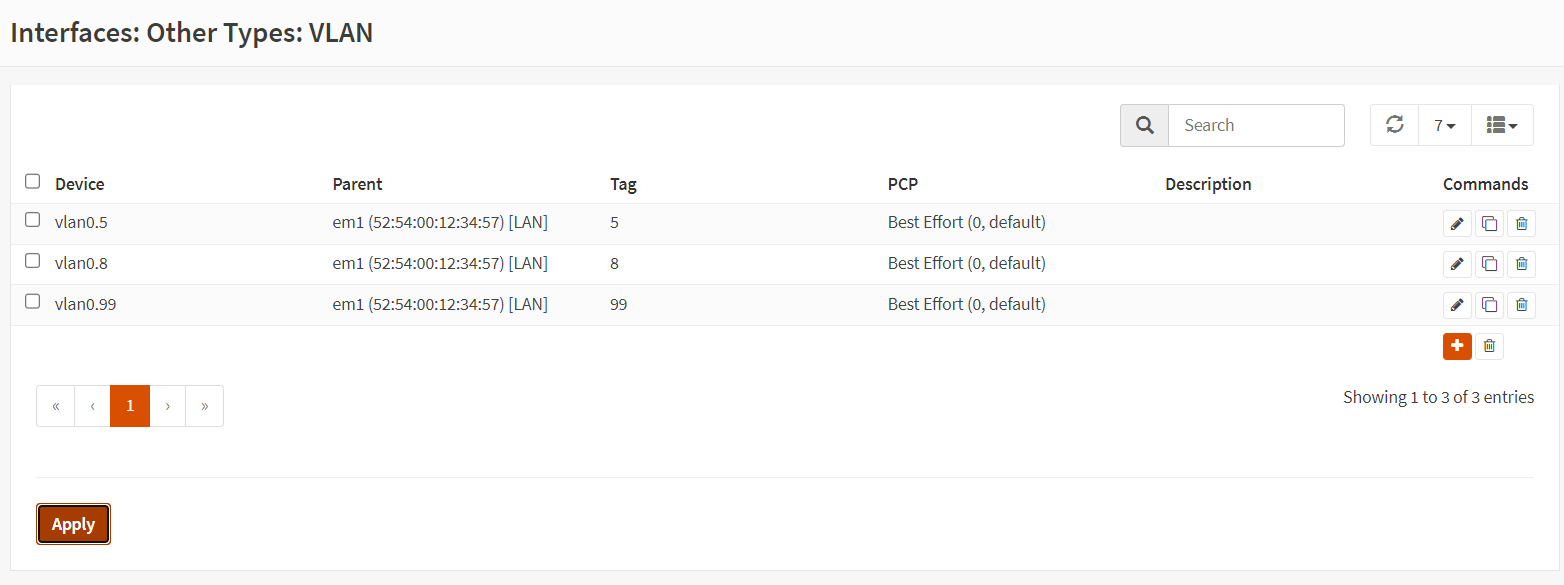
\includegraphics[width=0.93\textwidth]{5_interfaces_other_types_vlan.png}

      \item Go to \textbf{Interfaces: Assignments} and assign VLAN devices to OPT1, OPT2, and and OPT3.

      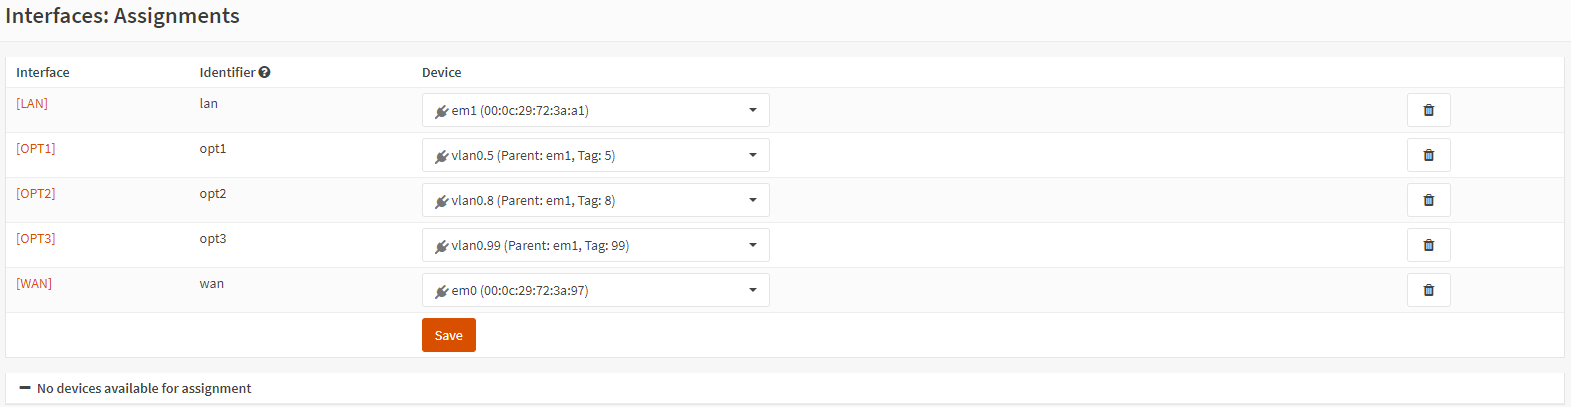
\includegraphics[width=0.93\textwidth]{5_interfaces_assignments}

      \item Go to \textbf{Interfaces: [OPT1]}.
      \begin{enumerate}
        \item Select \textbf{Enable Interface}.
        \item In the \textbf{IPv4 Configuration Type} list, select \textbf{Static IPv4}.
        \item In the \textbf{IPv4 address} box, \verb|enter 10.5.0.1/24|.
      \end{enumerate}
      \item Repeat step (c) for interfaces OPT2 and OPT3, but use IPv4 addresses
      \verb|10.8.0.1/24| and \verb|10.99.0.1/24| respectively.

      \item \textbf{Steps}

      Go to \textbf{Services: ISC DHCPv4: [OPT1]}.
      \begin{enumerate}
        \item Select \textbf{Enable DHCP server on the OPT1 interface}.
        \item In the \textbf{Range} boxs, enter \verb|10.5.0.2| in the \textbf{from} box and \verb|10.5.0.254| in the \textbf{to} box.
        \item in the \textbf{DNS servers} boxes, enter \verb|8.8.8.8| and \verb|8.8.4.4|.
      \end{enumerate}

      \item Repeate step (e) for interfaces OPT2 and OPT3, but use ranges
      \verb|10.8.0.2-10.8.0.254| and \verb|10.99.0.2-10.99.0.254| respectively.
    \end{enumerate}

    \pagebreak
    \textbf{Result}

    \verb|eth0.5|

    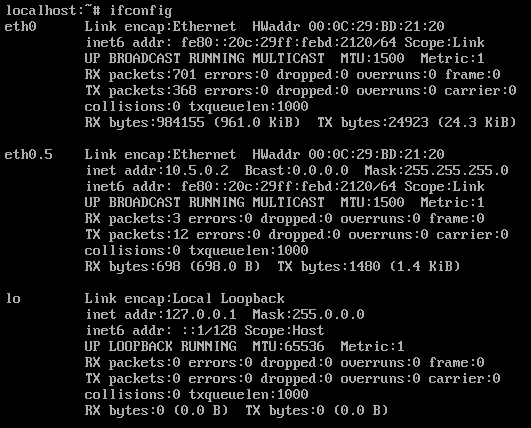
\includegraphics[width=0.7\textwidth]{5_eth0.5.png}

    \verb|eth0.8|

    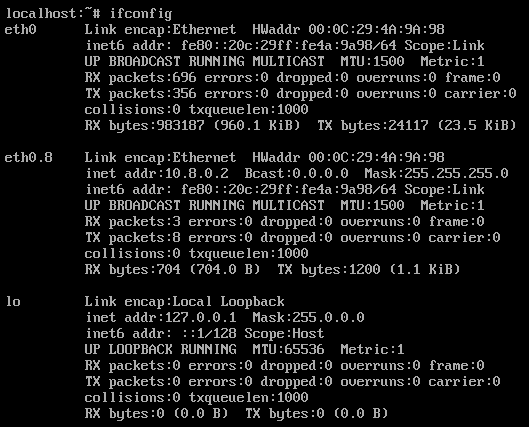
\includegraphics[width=0.7\textwidth]{5_eth0.8.png}

    \pagebreak
    \verb|eth0.99|

    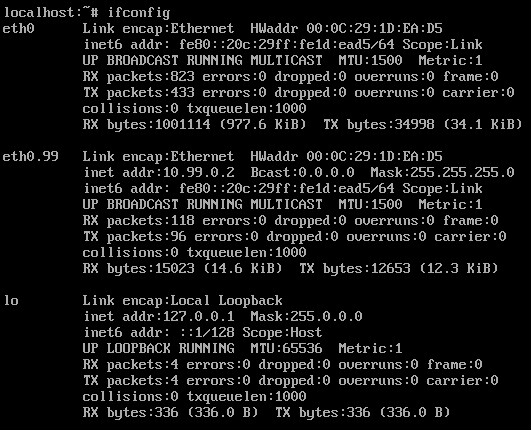
\includegraphics[width=0.7\textwidth]{5_eth0.99.png}

    \verb|cat /etc/resolv.conf|:

    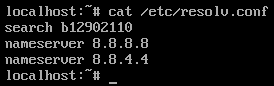
\includegraphics[width=0.4\textwidth]{5_etc_resolv.conf.png}

    \textbf{References}
    \begin{itemize}
      \item \href{https://hackmd.io/@chyijia/SJB7aW73p#/}{NASA 2024 OPNsense lab - HackMD}
    \end{itemize}

    \pagebreak
    \item
    \textbf{Steps}

    Go to \textbf{Firewall: Aliases} and add the aliases.
    \begin{itemize}
      \item
      \begin{itemize}
        \item \textbf{Name}: \verb|GOOGLE_DNS|
        \item \textbf{Type}: Host(s)
        \item \textbf{Content}: \verb|8.8.8.8|, \verb|8.8.4.4|
      \end{itemize}
      \item
      \begin{itemize}
        \item \textbf{Name}: \verb|ADMIN_PORTS|
        \item \textbf{Type}: Port(s)
        \item \textbf{Content}: \verb|22|, \verb|80|, \verb|443|
      \end{itemize}
      \item
      \begin{itemize}
        \item \textbf{Name}: \verb|CSIE_WORKSTATIONS|
        \item \textbf{Type}: Host(s)
        \item \textbf{Content}: \verb|ws1.csie.org|, \verb|ws2.csie.org|, \verb|ws3.csie.org|, \verb|ws4.csie.org|,\\ \verb|ws5.csie.org|
      \end{itemize}
    \end{itemize}

    \textbf{Result}

    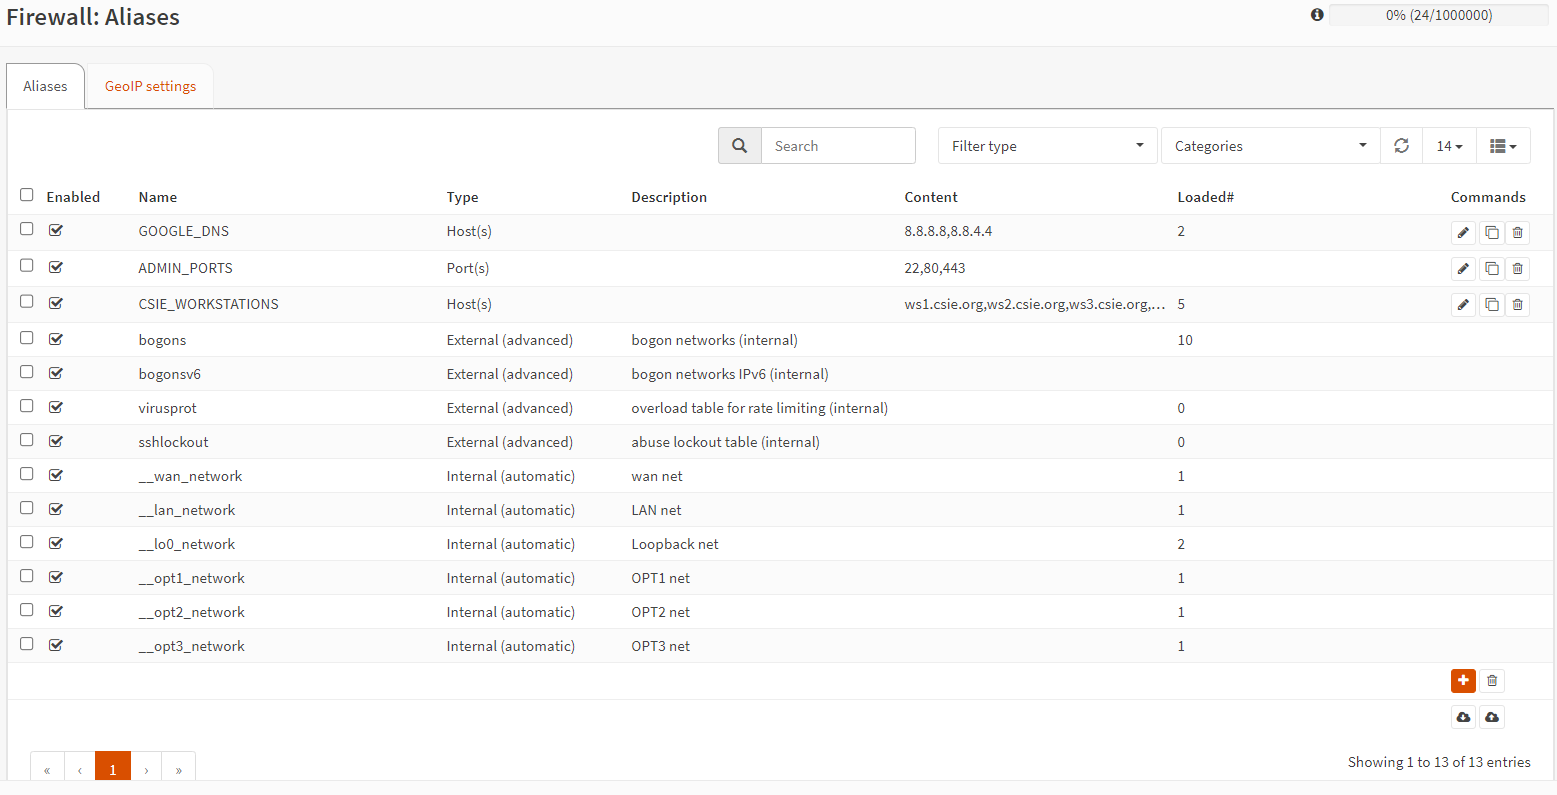
\includegraphics[width=0.93\textwidth]{6_firewall_aliases.png}

    \textbf{References}
    \begin{itemize}
      \item \href{https://docs.opnsense.org/manual/aliases.html}{Aliases — OPNsense  documentation}
    \end{itemize}

    \pagebreak
    \item
    \textbf{Steps}

    Go to \textbf{System: Settings: Administration}.
    \begin{enumerate}
      \item Select \textbf{Enable Secure Shell}.
      \item Select \textbf{Permit root user login}.
      \item Select \textbf{Permit password login}.
      \item In the \textbf{Listen Interfaces} list, select \textbf{WAN} and \textbf{OPT3}.
    \end{enumerate}

    \textbf{Result}

    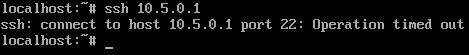
\includegraphics[width=0.7\textwidth]{7_ssh_vlan5.png}

    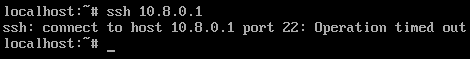
\includegraphics[width=0.7\textwidth]{7_ssh_vlan8.png}
%
%    \includegraphics[width=0.9\textwidth]{7_ssh_vlan99.png}

    \item
    \textbf{Steps}

    Go to \textbf{Firewall: Rules: OPT3} and add the following rules. (Note: Traffic from OPT1 and OPT2 are blocked by default.)
    \begin{itemize}
      \item
      \begin{itemize}
        \item \textbf{Action}: Pass
        \item \textbf{Interface}: OPT3
        \item \textbf{Direction}: in
        \item \textbf{TCP/IP Version}: IPv4
        \item \textbf{Protocol}: any
        \item \textbf{Source}: any
        \item \textbf{Destination}: GOOGLE\_DNS
      \end{itemize}
      \item
      \begin{itemize}
        \item \textbf{Action}: Pass
        \item \textbf{Interface}: OPT3
        \item \textbf{Direction}: in
        \item \textbf{TCP/IP Version}: IPv4
        \item \textbf{Protocol}: any
        \item \textbf{Source}: any
        \item \textbf{Destination}: CSIE\_WORKSTATIONS
      \end{itemize}
      \item
      \begin{itemize}
        \item \textbf{Action}: Pass
        \item \textbf{Interface}: OPT3
        \item \textbf{Direction}: in
        \item \textbf{TCP/IP Version}: IPv4
        \item \textbf{Protocol}: TCP
        \item \textbf{Source}: any
        \item \textbf{Destination}: This Firewall
        \item \textbf{Destination port range}: from: ADMIN\_PORTS, to: ADMIN\_ports
      \end{itemize}
    \end{itemize}

    \clearpage
    \textbf{Result}

    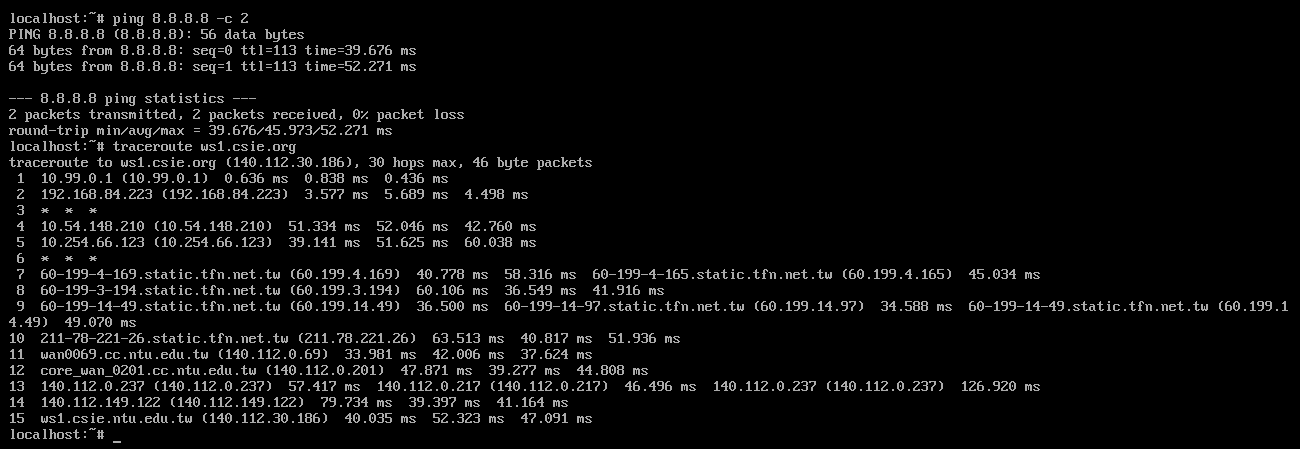
\includegraphics[width=0.93\textwidth]{8_ping_traceroute.png}

    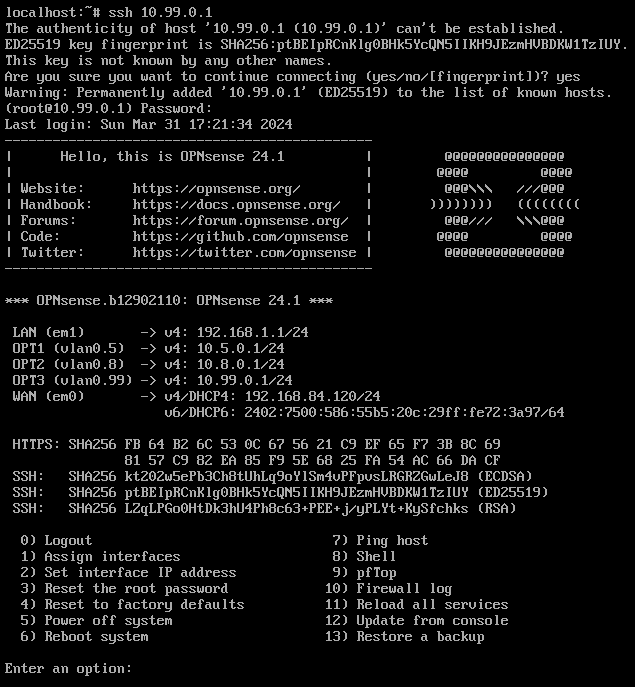
\includegraphics[width=0.8\textwidth]{8_ssh.png}

    \textbf{References}
    \begin{itemize}
      \item B12902040 黃昱翔
    \end{itemize}

    \pagebreak
    \item
    \textbf{Steps}
    \begin{enumerate}
      \item Go to \textbf{Firewall: Rules: OPT1} and add the following rule.
      \begin{itemize}
        \item \textbf{Action}: Pass
        \item \textbf{Interface}: OPT1
        \item \textbf{Direction}: in
        \item \textbf{TCP/IP Version}: IPv4
        \item \textbf{Protocol}: ICMP
        \item \textbf{ICMP type}: any
        \item \textbf{Source}: OPT1 net
        \item \textbf{Destination}: OPT2 net
      \end{itemize}
      \item Go to \textbf{Firewall: Rules: OPT2} and add the following rules.
      \begin{itemize}
        \item
        \begin{itemize}
          \item \textbf{Action}: Pass
          \item \textbf{Interface}: OPT2
          \item \textbf{Direction}: in
          \item \textbf{TCP/IP Version}: IPv4
          \item \textbf{Protocol}: ICMP
          \item \textbf{ICMP type}: Echo Reply
          \item \textbf{Source}: OPT2 net
          \item \textbf{Destination}: OPT1 net
        \end{itemize}
        \item
        \begin{itemize}
          \item \textbf{Action}: Block
          \item \textbf{Interface}: OPT2
          \item \textbf{Direction}: in
          \item \textbf{TCP/IP Version}: IPv4
          \item \textbf{Protocol}: ICMP
          \item \textbf{ICMP type}: Echo Request
          \item \textbf{Source}: OPT2 net
          \item \textbf{Destination}: OPT1 net
        \end{itemize}
      \end{itemize}
    \end{enumerate}

    \textbf{Result}

    On \verb|10.5.0.2|, ping \verb|10.8.0.2|:

    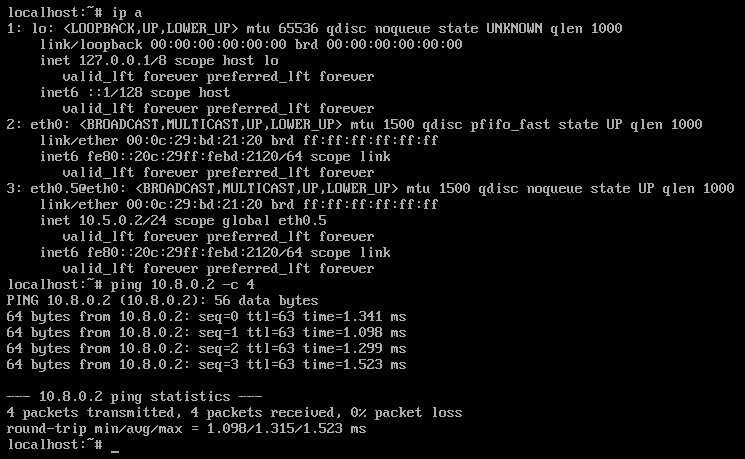
\includegraphics[width=0.8\textwidth]{9_vlan5_to_vlan8.png}

    On \verb|10.8.0.2|, ping \verb|10.5.0.2|:

    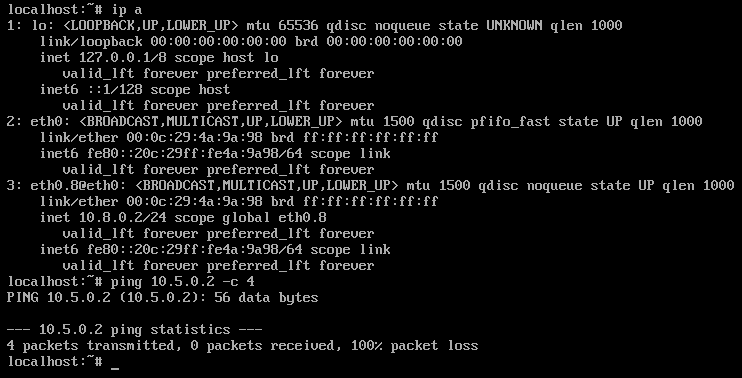
\includegraphics[width=0.8\textwidth]{9_vlan8_to_vlan5.png}

    \item
    \textbf{Steps}
    \begin{itemize}
      \item Go to \textbf{Firewall: Settings: Schedules} and add the folowing schedule.
      \begin{itemize}
        \item \textbf{Name}: 2024-03-14
        \item \textbf{Month}: March\_24
        \item \textbf{Day}: 14
        \item \textbf{Time}: Start time: 0:00, Stop time: 23:59
      \end{itemize}
      \item Go to \textbf{Firewall: Rules: OPT1} and add the following rule
      as the first rule.
      \begin{itemize}
          \item \textbf{Action}: Block
          \item \textbf{Interface}: OPT1
          \item \textbf{Direction}: in
          \item \textbf{TCP/IP Version}: IPv4+IPv6
          \item \textbf{Protocol}: any
          \item \textbf{Source}: any
          \item \textbf{Destination}: any
          \item \textbf{Schedule}: 2024-03-14
      \end{itemize}
    \end{itemize}

    \pagebreak
    \item \textbf{Observations}
    \begin{itemize}
      \item The graph's y-axis scales automatically according to the maximum
      value during the time span.
      \item The graph samples data at regular intervals, and the data seems
      to be the average over a few seconds.
      \item Each interface is represented with a different color.
    \end{itemize}


    \textbf{Steps}
    \begin{itemize}
      \item Install:
      \begin{verbatim}
apk add hping3 --update-cache --repository \
  http://dl-cdn.alpinelinux.org/alpine/edge/testing
      \end{verbatim}
      \item 100kbps: \verb|hping3 -d 1250 -i u100000 192.168.1.1|
      \item 1Mbps: \verb|hping3 -d 12500 -i u100000 192.168.1.1|
      \item 10Mbps: \verb|hping3 -d 15000 -i u10000 192.168.1.1|
      \item 50Mbps: \verb|hping3 -d 50000 -i u5000 192.168.1.1|
    \end{itemize}

    \textbf{Result}

    100kbps:

    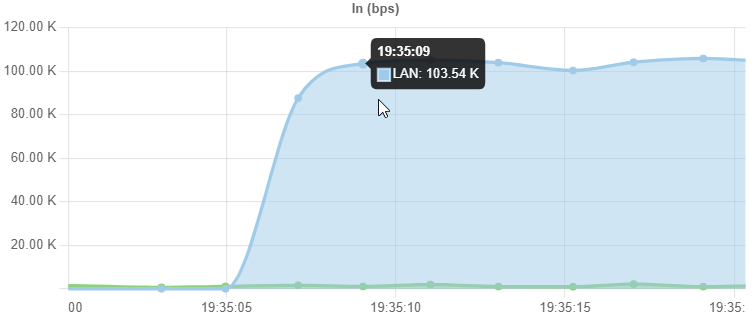
\includegraphics[width=0.7\linewidth]{11_100kbps.png}

    1Mbps:

    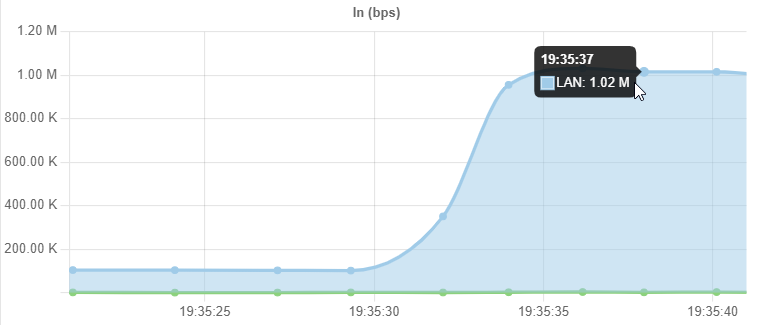
\includegraphics[width=0.7\linewidth]{11_1Mbps.png}

    \clearpage
    10Mbps:

    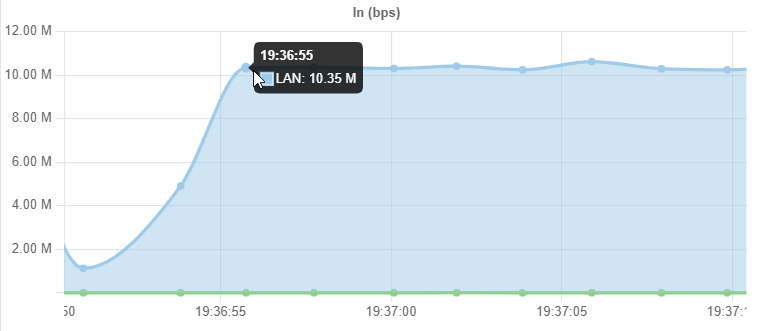
\includegraphics[width=0.7\linewidth]{11_10Mbps.png}

    50Mbps:

    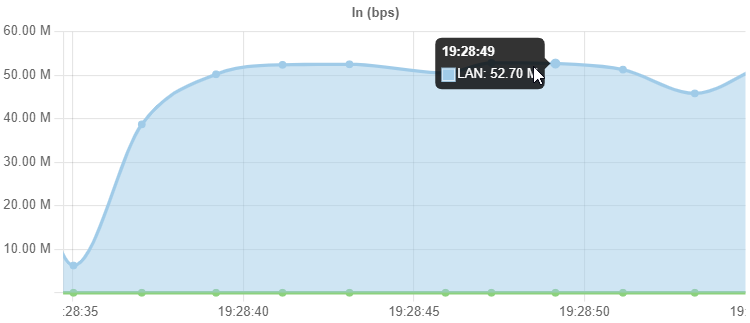
\includegraphics[width=0.7\linewidth]{11_50Mbps.png}

    \textbf{References}
    \begin{itemize}
      \item \href{https://pkgs.alpinelinux.org/package/edge/testing/x86_64/hping3}{Alpine Linux packages - hping3}
      \item \href{https://unix.stackexchange.com/questions/371762/alpine-linux-unable-to-install-hping-error-unsatisfiable-constraints}{software installation - Alpine Linux unable to install hping; ERROR: unsatisfiable constraints - Unix \& Linux Stack Exchange}
      \item \href{https://linux.die.net/man/8/hping3}{hping3(8) - Linux man page}
      \item \href{https://docs.opnsense.org/manual/reporting_traffic.html}{Reporting: Traffic — OPNsense  documentation}
      \item \href{https://jyos-sw.medium.com/know-about-hping3-linux-tool-4fdcac05a493}{Know about hping3 linux tool. hping3 is a network tool that can be… | by Jyothi | Medium}
    \end{itemize}
  \end{enumerate}
\end{document}
